\section{Simulation Results}
\label{sec:simulation}
The simulation results are consistant across all the PARSEC benchmarks. The reason for this consistancy is due to the similarity of the memory traces across the benchmarks. Given sufficient memory overhead, we see that we consistantly achieve a roughly 25\% improvement over the baseline simulation. We generally find that the Coding Scheme I performs the best out of the proposed schemes. 

\subsection{PARSEC Results}

The proposed memory system performs consistantly across the PARSEC benchmarks, and the three proposed schemes yield similar results. Figure~\ref{fig:dedup_results} shows the simulation results for the dedup benchmark. The plot shows that the number of CPU cycles is reduced by between 83\% and 73\% once a sufficient amount of memory is provided to the memory system. 

These results were simulated using a memory bank partition of .05. We observe that the performance remains consistant for values of $\alpha > .1$. The reason for this is that there are two heavily accesses memory bands in each of the PARSEC benchmarks. Once the memory system is able to encode both of these regions, the benefits of the memory system are fully realized. At an $\alpha = .1$, the memory system finds and encodes the two heavily accesses memory bands. This is made more evident by observing the number of times the memory system choses a new region to encode. When $\alpha = .05$, the number of switches is very high because the memory system vasilates between the two most heavily accesses bands. When $\alpha = .1$, the number of switches is nearly zero because the memory system can only select two memory regions to encode, and it seldom has a reason to switch away from the two heavily accessed bands. We see small numbers of switches when $\alpha = {.25, .5}$ because the memory system is encoding less heavily accesses memory bands.

\begin{figure}[htbp]
		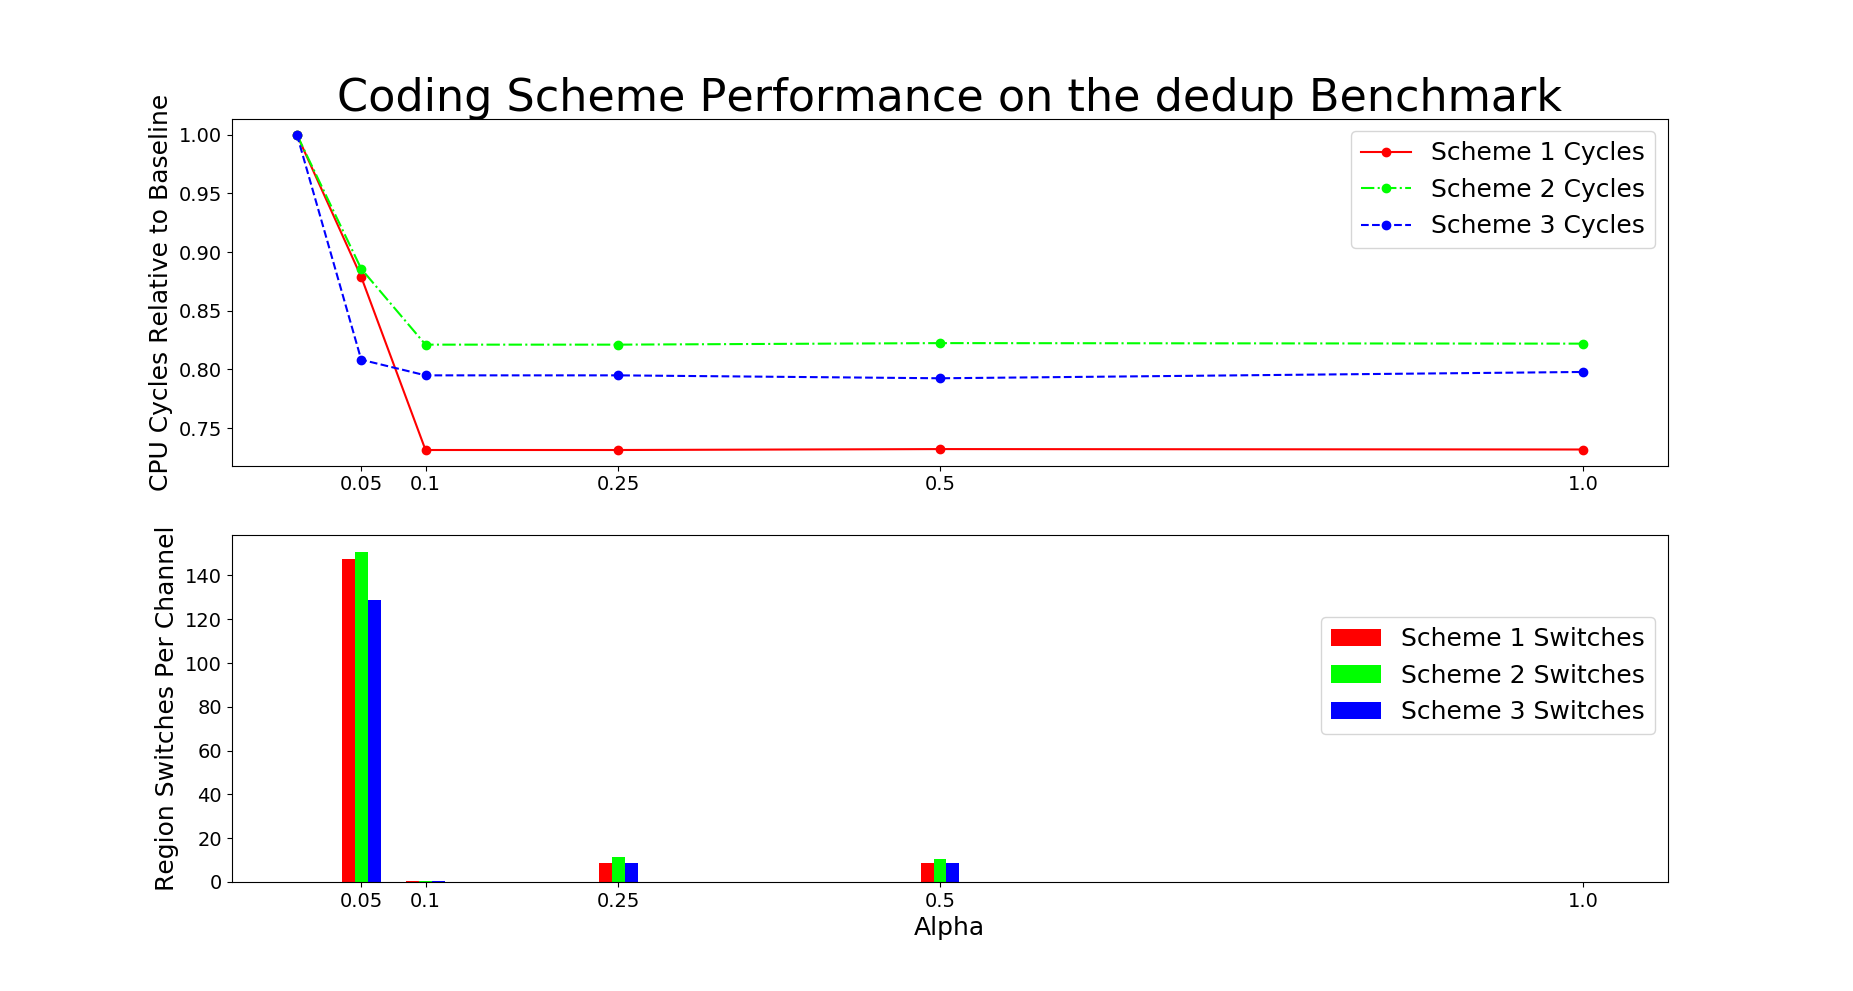
\includegraphics[width=\linewidth]{fig/dedup_benchmark_results.png}
		\caption{The simulation results for the dedup PARSEC benchmark. The line plot represents the number of CPU cycles needed and the bar plot represents the number of tiems the dynamic coding unit chooses to encode a new memory region. The results from the other PARSEC benchmarks are very similiar to those seen here.}
		\label{fig:dedup_results}
\end{figure}
\begin{figure}[htbp]
		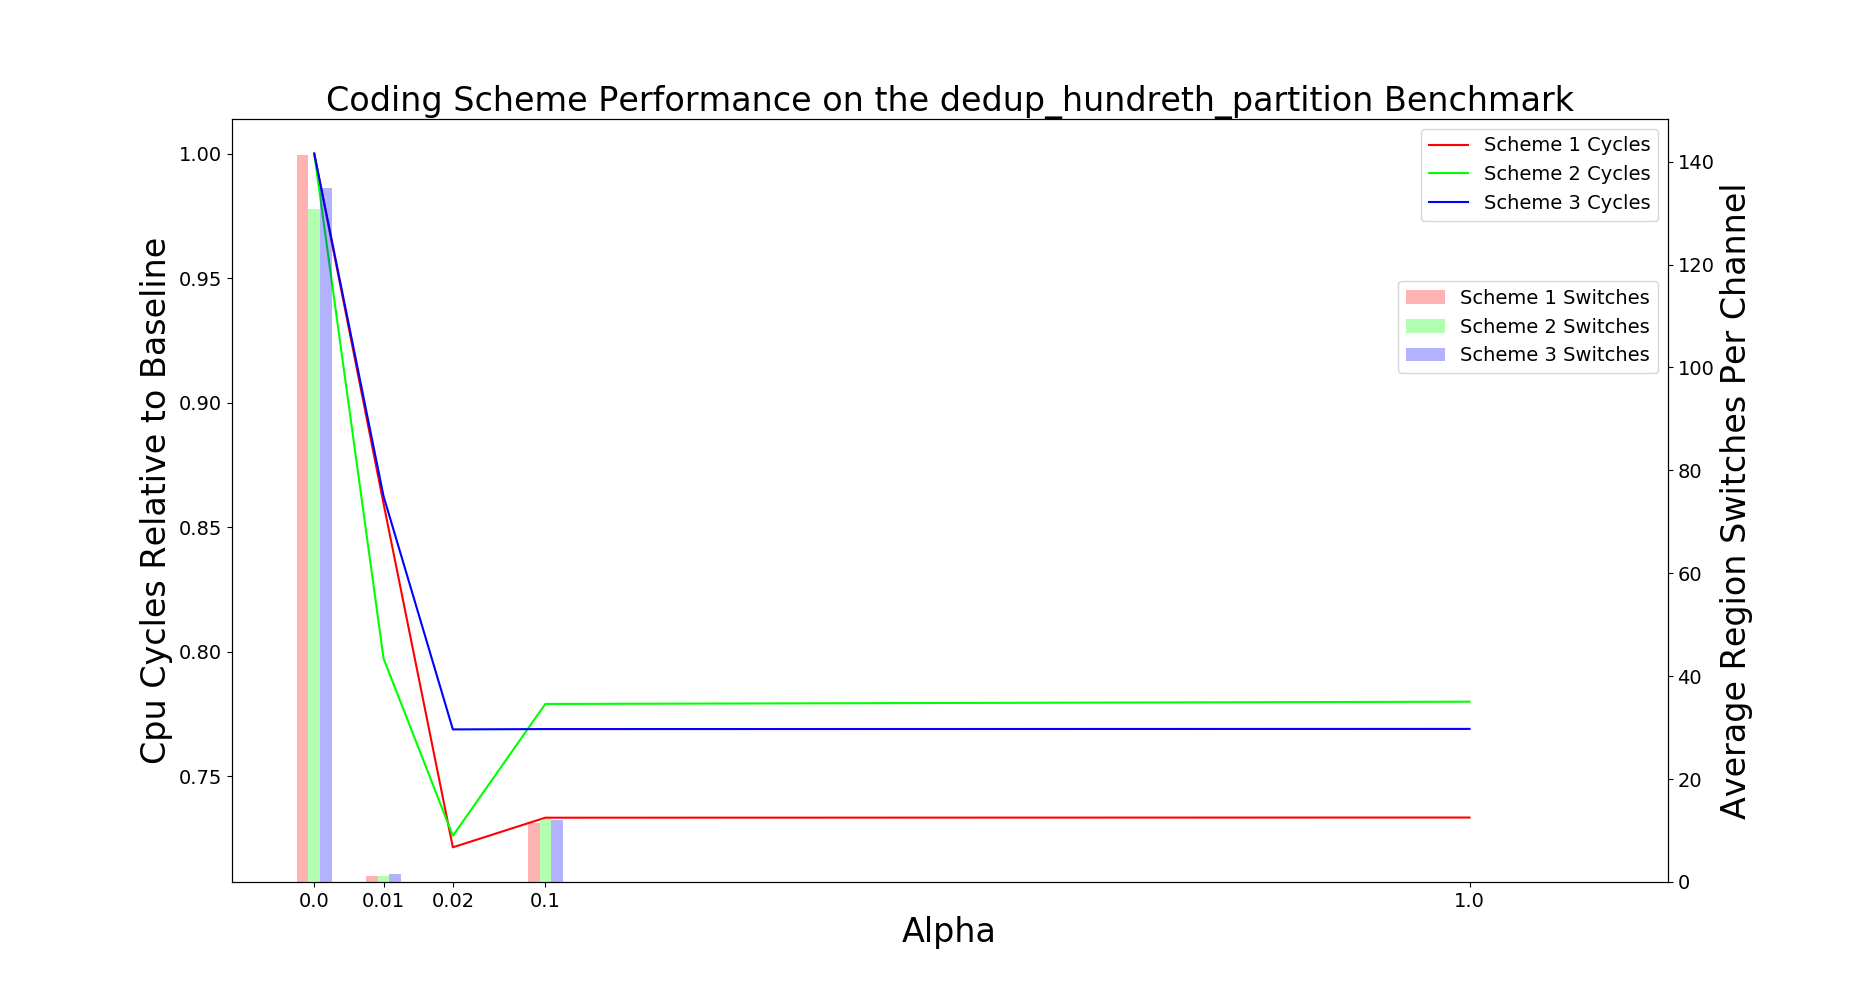
\includegraphics[width=\linewidth]{fig/dedup_hundreth.png}
		\caption{The simulation results for the same trace simulated in Figure~\ref{fig:dedup_results} but with a memory partition coefficient $r = .01$}
		\label{fig:dedup_hundreth}
\end{figure}

The heavily accesses memory bands are narrow, so decreasing the memory bank partition to allows us to lower $\alpha$ and see no decrease in performance. This is demonstrated by Figure~\ref{fig:dedup_hundreth}. Here, it is shown that we can reduce 5 times more than the previous simulation. This is achieved by decreasing the memory partition coefficient $r$ from .05 to .01.


\subsection{PARSEC Augmentation}
Because the PARSEC benchmarks are homogenous in structure, we chose to augment them in order to observe how the proposed memory system performs in more scenarios. The PARSEC benchmarks were augmented in two ways. The first augmentation is to split the memory bands observed in Figure~\ref{fig:dedup_whole} and Figure~\ref{fig:dedup_dense} into a greater number of bands. The second augmentation was to ramp the memory bands over time. A visualization of the augmented traces can be seen in Figure~\ref{fig:vips_split} and~\ref{fig:vips_ramp}

\begin{figure}[htbp]
		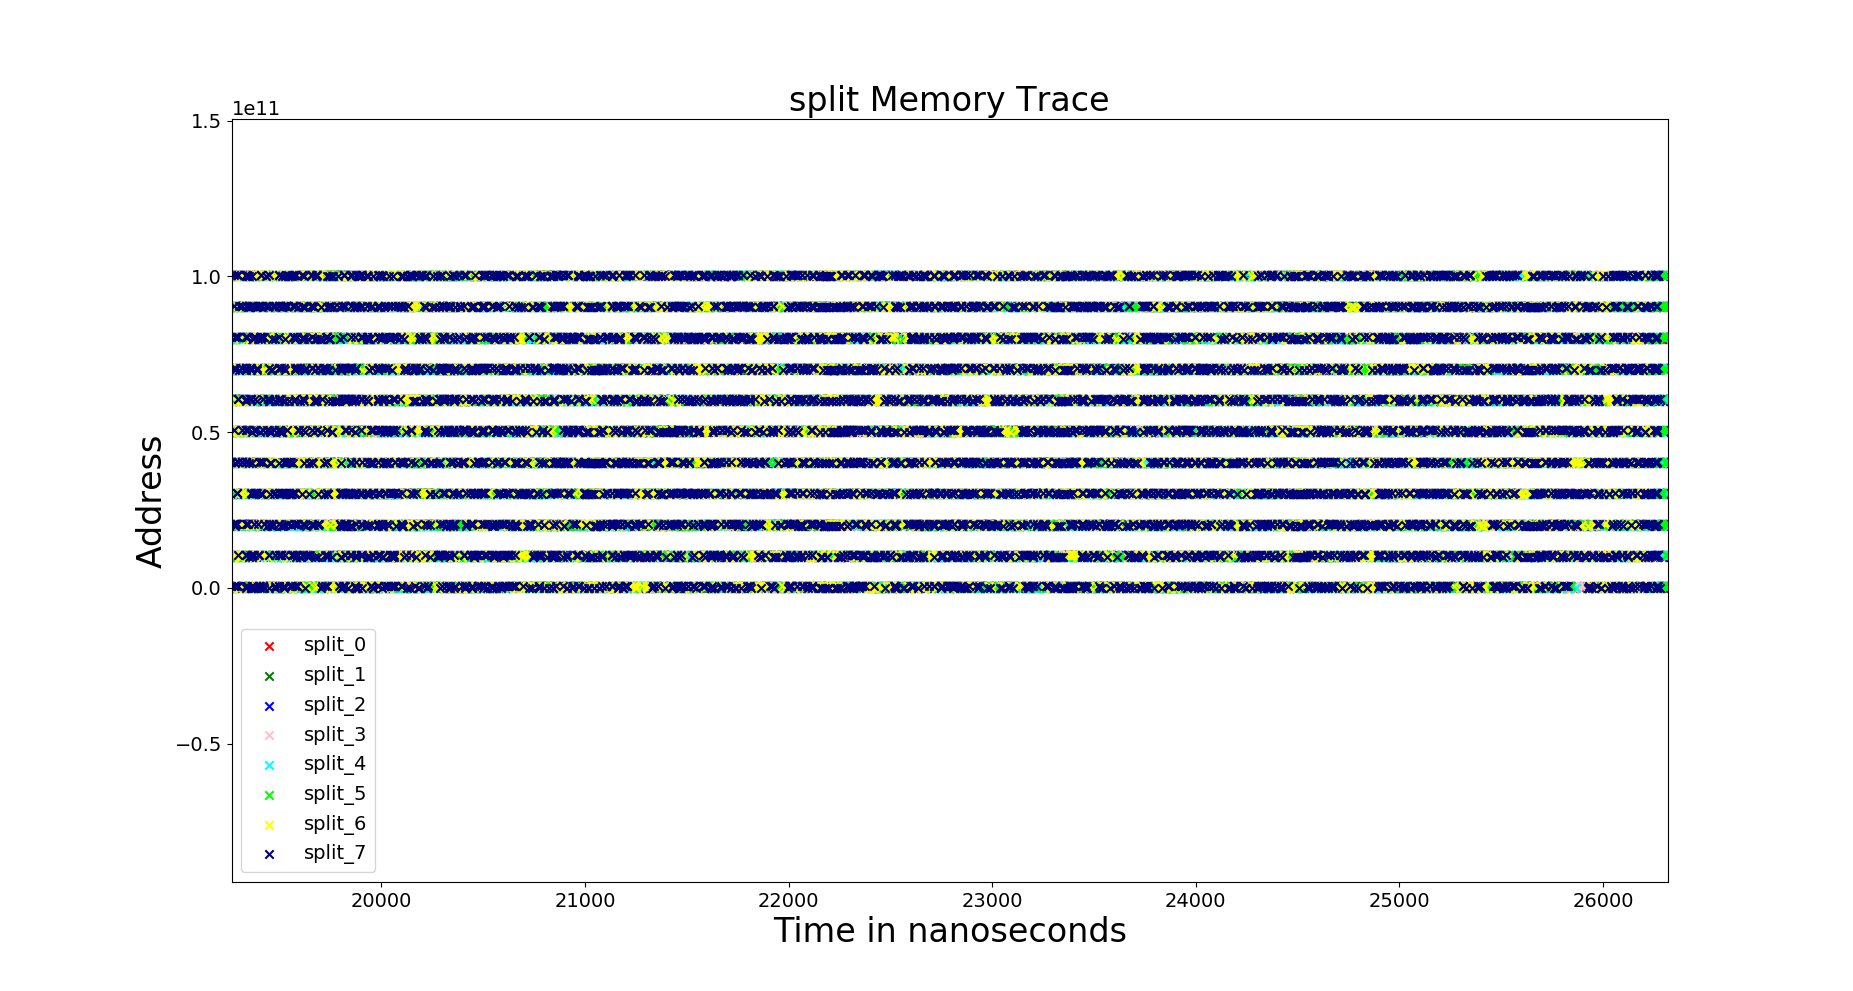
\includegraphics[width=\linewidth]{fig/vips_split.png}
		\caption{The vips benchmark after the major memory access bands were split into a greater number of bands}
		\label{fig:vips_split}
\end{figure}


\begin{figure}[htbp]
		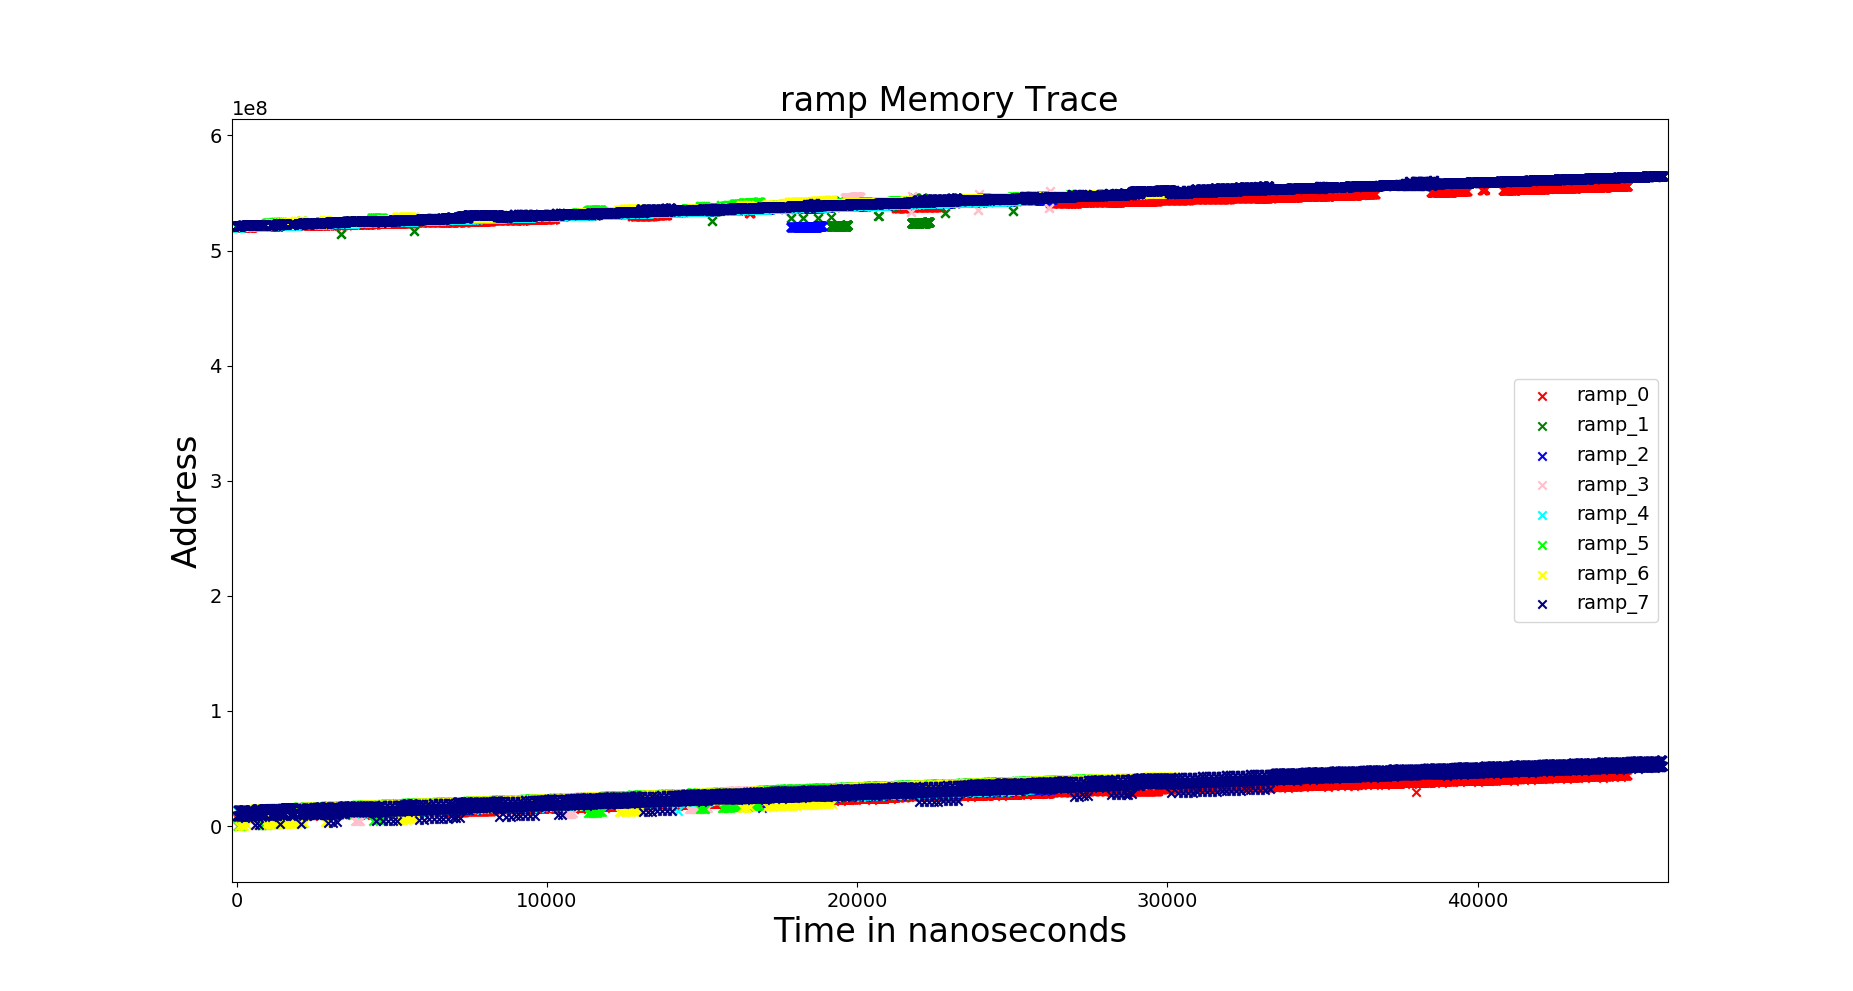
\includegraphics[width=\linewidth]{fig/vips_ramp.png}
		\caption{The vips benchmark after a ramp was added to the major memory bands}
		\label{fig:vips_ramp}
\end{figure}

\subsection{Augmented PARSEC Results}

The augmented PARSEC results significantly impact the Ramulator simulation results. Increasing the number of memory bands by splitting the dense bands results in an increased memory requirement to see improved performance. Introducing a ramp to the memory bands decreases the efficacy of the proposed memory system across all values of $\alpha$.

Figure~\ref{fig:vips_split_result} shows the results from the split augmentation pictured in Figure~\ref{fig:vips_split_result}. When there are large number of memory bands, the proposed memory system can achieve the same performance as when there are fewer memory bands given an increased memory allowance. Note that the simluation results in Figure~\ref{fig:vips_split_result} can be achieved using less memory by decreasing the memory partition coefficient. The memory partition coefficient used here is $r = 0.05$, but as shown in Figures ~\ref{fig:dedup_results} and ~\ref{fig:dedup_hundreth} lowering the memory partition coefficient allows a lowering of $\alpha$ while achieving the same performance.

Figure~\ref{fig:vips_ramp_result} shows the results of the ramp augmentation pictured in Figure~\ref{fig:vips_ramp_result}. The performance of the proposed memory system is less for this trace. The number of memory region switches shows that the memory system struggles to handle the constantly changing location of the heavily accessed memory regions. In the other simulator results, we see that the number of memory region switches decreases as a function of $\alpha$. The reason for this is that the memory system locates the heavily accessed memory regions and rarely switches away from them. Here, the memory system is constantly attempting to catch up with the heavily accessed memory region. {\color{blue}We note that the ramp covers a very large number of memory addresses, so the decrease in performance we observe would only effect programs which use very large portions of memory.} 

\begin{figure}[htbp]
		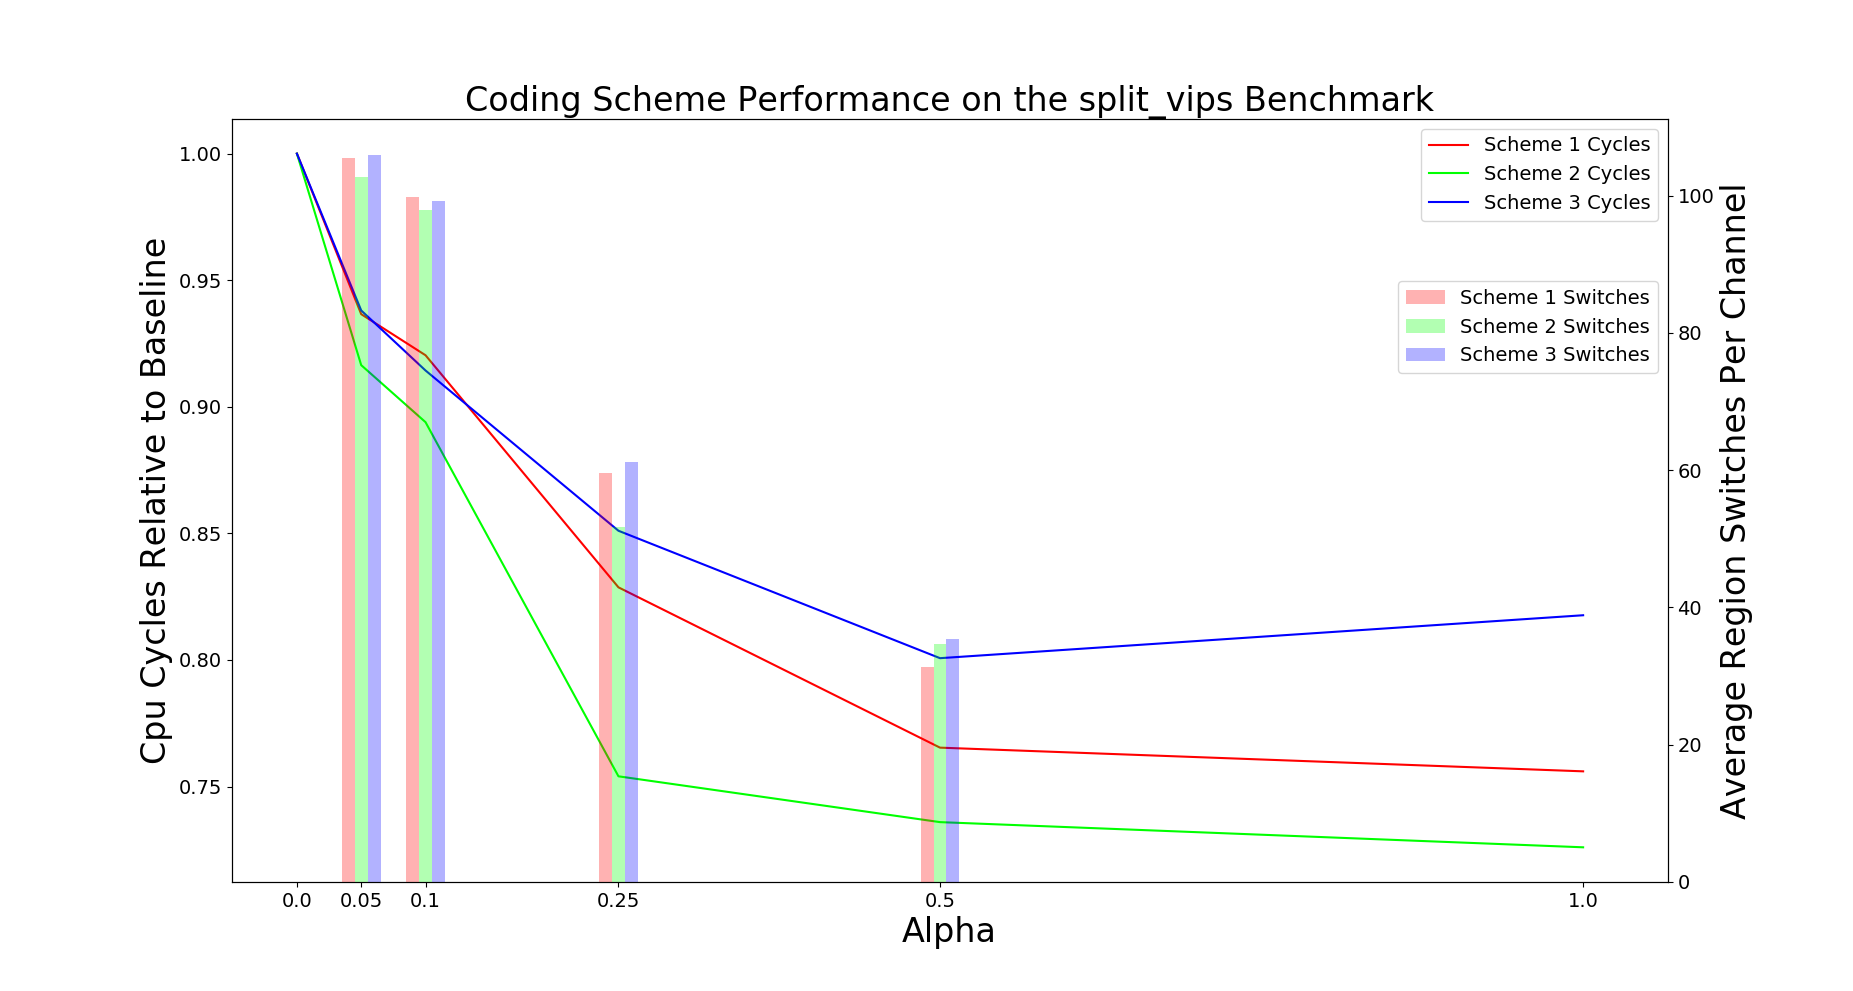
\includegraphics[width=\linewidth]{fig/vips_split_results.png}
		\caption{The simulation results of the augmented vips trace pictured in Figure~\ref{fig:vips_split}}
		\label{fig:vips_split_result}
\end{figure}

\begin{figure}[htbp]
		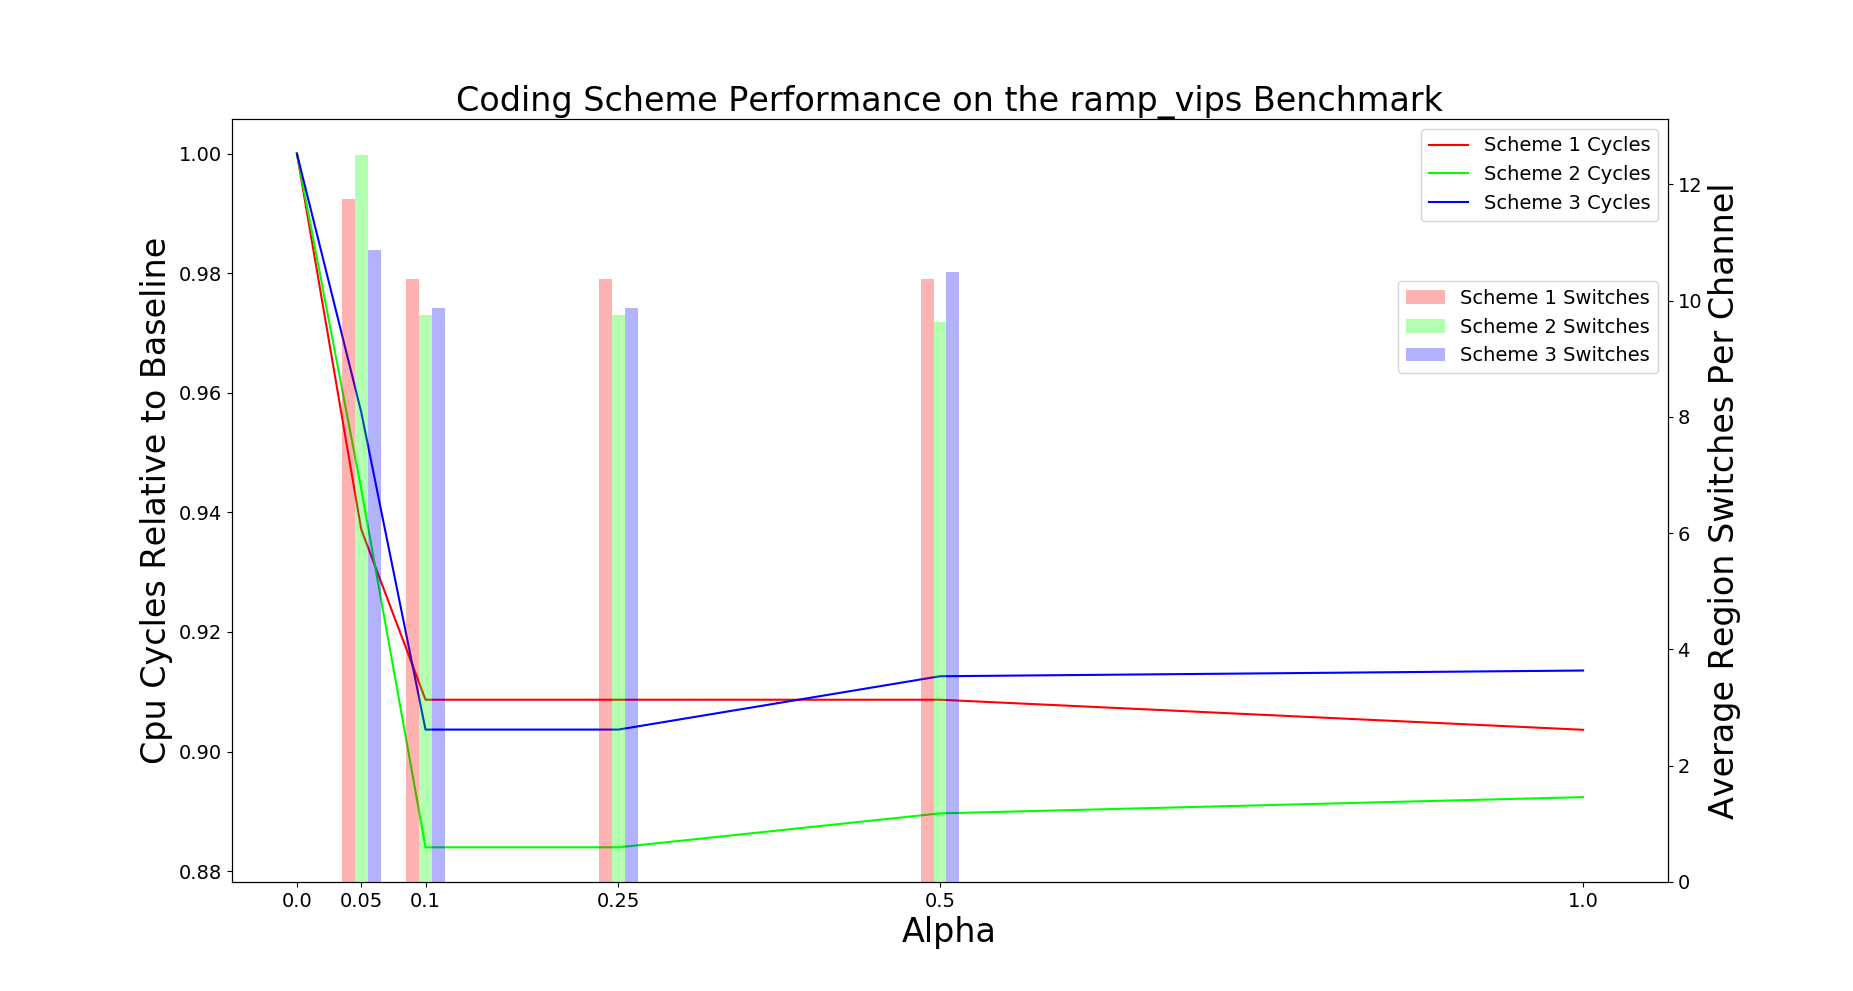
\includegraphics[width=\linewidth]{fig/vips_ramp_results.png}
		\caption{The simulation results of the augmented vips trace pictured in Figure~\ref{fig:vips_ramp}}
		\label{fig:vips_ramp_result}
\end{figure}

\subsection{Design Parameters}
\Matt{This section is old and needs to be updated to reflect our shift in focus away from LTE/UMTS}
In this section, we discuss various parameters that we consider 
%in this phase of the project 
to design and simulate the efficient code storage in this project. \\
\textit{Memory overhead}: 
%The gains of multiple accesses to a memory bank every cycle comes with an 
%associated cost. 
The crucial cost in coded memory system is to store the compressed redundancy or 
the codes. The extra memory space used to store these codes should limit to 
15$\%$ of the overall memory.\\
\textit{Memory size}: The memory size and the parity storage size decide the 
code function to be used to essentially compress the redundant data. This design 
considers a portion of memory to be coded. \\ \textit{Memory Banks}: The memory 
banks essentially are the units which store the data. We consider the code 
design for 8 memory banks. We consider the memory banks addressed with Least 
Significant Bits (LSBs) of the address. The last 3 bits of the address decide 
which bank, the memory address belongs to and the rest of the MSBs decide the 
row location within the bank.\\ \textit{Cache line size}: The memory accesses 
are bundled in a burst as a cache line is evicted and is requested to be 
replaced by the cores. The cache controller thus requests a cache line which is 
a starting address and the length of the cache line. In this design, we consider 
cache line size of 128 bytes and 256 bytes. However, each core can potentially 
have a different cache line size and the concept of coding could be extended for 
various sizes.\\ \textit{Element size}:  Each memory location in a memory bank 
stores 256 bit of data. This essentially relates to decoding/understanding the 
address access request to the memory bank. The cores request memories to be read 
or written for multiple elements. For example, a core with 128 bytes of cache 
line would request 4 elements of read/write for each cache line. The shared 
traces have two different request patterns, for 128 bytes and for 256 bytes. \\
\textit{Number of Cores}: This parameter refers number of cores making access to 
the memory controller. This parameter is not used in the design of the coding 
scheme. However, we validate the design using the 6 core access trace shared 
with us for LTE and UMTS. \\
\textit{Access rate}: This is the average rate at which the memory controller 
executes the reads/writes to the memory banks. In this design, we consider 1.54 
ns as the access rate. This would mean that the clock rate to memory would be at 
650MHz. This parameter is required to simulate the performance for the shared 
traces.  
